\documentclass[a4paper,11pt]{article}

\usepackage{caratula}
\usepackage[spanish, activeacute]{babel}
\usepackage{amsfonts}
\usepackage{color}
\usepackage{graphicx}
\usepackage{float}
%\usepackage{algorithm2e}
% \usepackage{algpseudocode}
\usepackage{ucs}
\usepackage[utf8x]{inputenc}
\usepackage{fontenc}
\usepackage{listings}
\usepackage{amssymb}
\usepackage{amsmath}
%~ \usepackage{slashbox}
\usepackage{url} 
\usepackage[margin=2cm]{geometry}
\usepackage[bookmarks=true]{hyperref}

\renewcommand{\labelitemi}{}
\renewcommand{\labelitemii}{}
\renewcommand{\labelitemiii}{}
\renewcommand{\labelitemiv}{}

\newcommand\tactica[1]{ \textcolor{red}{#1}}


\begin{document}

\documentclass[a4paper,10pt]{article}
\usepackage{caratula}
\usepackage{a4wide}

%opening
\begin{document}
\titulo{Trabajo pr\'actico Nro. 1 Reentrega}
\fecha{29/06/2010}
\materia{Ingenier\'ia de Software I}
\integrante{Facundo Carrillo}{693/07}{facu.zeta@gmail.com}
\integrante{Rodrigo Casta\~{n}o}{602/07}{castano.rodrigo@gmail.com}
\integrante{Agustina Ciraco}{630/06}{agusciraco@gmail.com}
\integrante{Mart\'in De Micheli}{523/07}{shmdm7@gmail.com}
\integrante{Federico Pousa}{221/07}{fedepousa@gmail.com}

\maketitle

\end{document}

 %1 Carátula + Abstract.

\newpage

\tableofcontents

\newpage 

%Hay que agregar casos de uso del TP1 muchos, tambien tiene muchas correciones 
\section{Casos de Uso}

A continuaci\'on se presentan los principales casos de uso del sistema.
Se presentan las principales interacciones que hay desde el exterior(votantes, rectorado, partidos pol\'iticos) con el sistema.

\begin{itemize}
\item Un usuario quieren ingresar al sistema
\begin{center}
\begin{tabular}{ll}
Actor & Votante \\
\hline
Pre condición & Ninguna \\
\hline
Pos condición & El usuario se encuentra autenticado. \\
\hline
\end{tabular}
\medskip
\begin{tabular}{c p{4cm}|p{4cm}}
 & Curso normal & Curso alternativo \\
 1. & El votante indica su nombre de usuario y contraseña &  \\
 2. & Si los datos son correctos el usuario recibe una confirmación de que su nombre de usuario y contraseña son correctos & Si los datos son incorrectos el usuario recibe un mensaje de error indicándo que la combinación de nombre de usuario y contraseña es incorrecta \\
 3. & Se muestra la interfaz de voto electrónico & Ir al fin del caso de uso \\
4. & Fin del caso de uso& \\ 
\end{tabular}
\end{center}

\bigskip
\item Un usuario quiere emitir un voto v\'alido.
\begin{center}
\begin{tabular}{ll}
Actor & Votante \\
\hline
Pre condición & El usuario se encuentra autenticado \\
\hline
Pos condición & Se registra correctamente el voto del usuario \\
\hline
\end{tabular}
\medskip
\begin{tabular}{c p{4cm}|p{4cm}}
 & Curso normal & Curso alternativo \\
 1. & Se muestra ante el usuario la lista de candidatos &   \\
 2. & El usuario selecciona el candidato de su preferencia &   \\
 3. & Se pide confirmación al usuario mostrando claramente qué candidato ha elegido &   \\
 4. & El votante confirma su selección & Si el usuario no confirma, se descarta la selección del usuario  \\
 5. & Se le informa al usuario que se ha enviado a su e\-mail el certificado del voto & Ir al fin del caso de uso \\
 6. & Fin del caso de uso & \\
\end{tabular}
\end{center}

\bigskip
\item Fiscalizaci\'on de los resultados parciales.
\begin{center}
\begin{tabular}{ll}
Actor & El usuario del fiscalizador \\
\hline
Pre condición & El usuario se encuentra autenticado \\
\hline
Pos condición & Se entregan resultados parciales \\
\hline
\end{tabular}
\medskip
\begin{tabular}{c p{4cm}|p{4cm}}
 & Curso normal & Curso alternativo \\
 1. & Se muestran opciones de resultados parciales por facultad con votaciones abiertas &   \\
 2. & El usuario selecciona el resultado parcial a observar &   \\
 3. & Fin del caso de uso & \\
\end{tabular}
\end{center}


\bigskip
\item El rectorado quiere enviar nuevos reglamentos a las facultades.
\begin{center}
\begin{tabular}{ll}
Actor & El usuario del rectorado \\
\hline
Pre condici\'on & El usuario se encuentra autenticado \\
\hline
Pos condici\'on & Las facultades reciben el nuevo reglamento \\
\hline
\end{tabular}
\medskip
% \begin{tabular}{c p{4cm}|p{4cm}}
%  & Curso normal & Curso alternativo \\
%  1. & Se muestran opciones de resultados parciales por facultad con votaciones abiertas &   \\
%  2. & El usuario selecciona el resultado parcial a observar &   \\
%  3. & Fin del caso de uso & \\
% \end{tabular}
\end{center}

\bigskip
\item Cambio de idioma en la interfaz de usuario.
\begin{center}
\begin{tabular}{ll}
Actor & Votante \\
\hline
Pre condición & El usuario se encuentra autenticado \\
\hline
Pos condición & La interfaz se presenta en el usuario elegido \\
\hline
\end{tabular}
\medskip
\begin{tabular}{c p{4cm}|p{4cm}}
 & Curso normal & Curso alternativo \\
 1. & El usuario selecciona la funcionalidad de modificar el idioma del sistema &   \\
 2. & El sistema despliega los diferentes idiomas disponibles &   \\
 3. & El usuario elije entre uno de las opciones disponibles & \\
 4. & El sistema modifica la interfaz del usuario con el idioma elegido & \\
 5. & Fin de caso de uso & \\
\end{tabular}
\end{center}



\bigskip
\item Conexi\'on desde diversas plataformas
\begin{center}
\begin{tabular}{ll}
Actor & Votante \\
\hline
Pre condición &  \\
\hline
Pos condición & El usuario ingresa al sistema \\
\hline
\end{tabular}
\medskip
\begin{tabular}{c p{4cm}|p{4cm}}
 & Curso normal & Curso alternativo \\
 1. & Un usuario quiere ingresar al sistema &   \\
 2. & El sistema chequea que la plataforma este soportada &   \\
 3. & Se procede con la autenticaci\'on del usuario & Se envia un mensaje al usuario que indica que la plaforma no esta soportada\\
 4. & Fin de caso de uso & \\
\end{tabular}
\end{center}

\bigskip
\item Auditabilidad de votantes
\begin{center}
\begin{tabular}{ll}
Actor & Usuario del rectorado \\
\hline
Pre condición & El usuario se encuentra autenticado\\
\hline
Pos condición & El rectorado sabe que votantes sufragaron \\
\hline
\end{tabular}
\medskip
\begin{tabular}{c p{4cm}|p{4cm}}
 & Curso normal & Curso alternativo \\
 1. & El rectorado selecciona la funcionalidad de auditabilidad &   \\
 2. & El sistema despliega la lista de la facultades disponibles &   \\
 3. & El recortorado elije la facultad que quiere auditar & Se envia un mensaje al usuario que indica que la plaforma no esta soportada\\
 4. & El sistema le envia al rectorado los votantes que sufragaron de la facultad seleccionada \\
 5. & Fin de caso de uso & \\
\end{tabular}
\end{center}



\end{itemize}

\newpage

%Parte opcional en realidad, hay que agregar los gantt y tratar vincular cada modulo del wbs con casos de uso
\section{Plan de proyecto}

\subsection{Etapas e Iteraciones}

El desarrollo del proyecto se elaborara en cuatro etapas: Elicitación, Diseño, Construcción y Transferencia. La etapa de elicitación contara con 2 iteraciones; el diseño con 3; la construcción con 4 y la transición con 2. Durante la etapa de elicitación se terminaran de consolidar los requerimientos funcionales y atributos de calidad de manera que queden definidos los drivers de la arquitectura. En la etapa de diseño se elaborara la especificación y modelos necesarios para comprender el funcionamiento del sistema. Durante la etapa de construcción es implementan los modulos especificados y en la etapa de transferencia se procede a realizar el deployment de las distintas piezas del sistema. 

La primera iteración comprenderá principalmente tareas de gestión y capacitación de los desarrolladores. Se tomó esta decisión porque identificamos varios intereses en conflicto y consideramos que es necesario establecer una prioridad entre ellos tan tempranamente como sea posible. Para hacer esto correctamente será necesario en primer lugar capacitar al equipo de desarrollo y de comunicación con los stakeholders en temas de seguridad. Priorizamos este tema en particular por haber sido considerado un atributo de calidad prioritario en el QAW y por la falta de capacitación del equipo en el mismo. 

Una vez realizada la capacitación será necesario identificar arquitecturas alternativas priorizando de manera diferente los distintos intereses en conflicto.

Contando con distintas alternativas arquitectónicas se realizará una serie de reuniones con los distintos stakeholders informándoles por qué los distintos intereses entran en conflicto desde un punto de vista tecnológico y en qué medida beneficia cada posible decisión arquitectónica a la concreción de un objetivo u otro.

Es crucial que la totalidad del equipo tenga conocimientos suficientes de seguridad para garantizar que no sean introducidas vulnerabilidades en módulos aparentemente no relacionados con el tema, por lo que la capacitación de los desarrolladores continuará y se solapará con las reuniones con los stakeholders. 

\subsubsection{Gantt}

En el primer diagrama mostramos como planeamos el proyecto a nivel general viendo así las distintas etapas y teniendo un tiempo estimado para las entregas. El tiempo estimado para
finalizar el desarrollo son 22 semanas.	

\begin{figure}[H]
 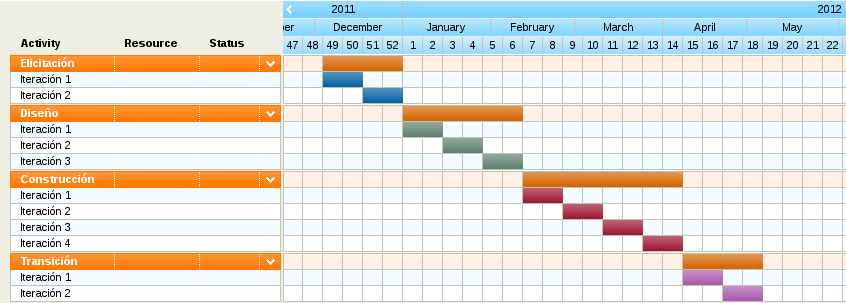
\includegraphics[scale=0.7]{./ganttetapas.png}
\end{figure}

En un segundo diagrama mostramos una de las iteraciones. Decidimos mostrar la primera iteración de la primera etapa, en donde se ven principalmente tareas de la etapa de elicitación. En la sección anterior comentamos de la importancia de esta etapa ya que es requerida para definir los \emph{Business Drivers} que se utilizaran para tomar decisiones en las siguientes etapas.

\begin{figure}[H]
\begin{center}
 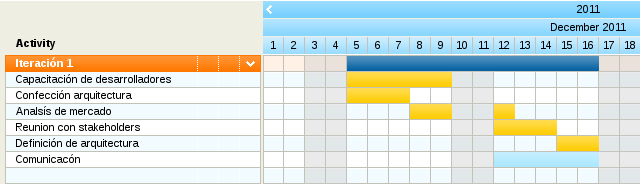
\includegraphics[scale=0.7]{./ganttiteracion.png}
\end{center}
\end{figure}

\renewcommand{\labelitemi}{$\tiny \blacksquare$}

Algunos puntos a destacar del diagrama:
\begin{itemize}
 \item Podemos ver que en esta iteración el equipo de desarrollo realizará dos tareas. Durante la primera semana se realiza la capacitación que consiste en instruir al equipo en diversos temas relacionados con seguridad ya que queremos minimizar problemas de este tipo. Durante la segunda semana pueden comenzar tareas de desarrollo realacionadas con los modulos relacionados a comunicación ya que se encuantra aislado al resto del sistema y tienen partes que no requieren de una arquitectura definida.
 \item El equipo de diseñadores se encarga inicialmente de realizar un arquitectura preliminar, para empezar a analizar alguno de los riesgos y problemas que nuestra arquitecutra deberá solucionar. Permite que se empiezen a analizar algunos de los problemas que se trataran con los stakeholders, y se veran que elementos externos serán requeridos.
 \item Luego habra una etapa de analisis de mercado para estar informados de las distintas tecnologias foraneas con las que nuestro proyecto podr\'a contar. Un punto clave para el proyecto por ejemplo es hacer un an\'alisis de servidores y proveedores de internet, ya que debemos manter una alta disponibilidad.
 \item Por último el equipo de diseñadores se encargara de reunirse con los stakeholders para terminar de definir la arquitectura. Para esto fue necesario tener una arquitectura preliminar, y haber investigado las tecnologias disponibles para consensuar aquellas a utilizar. 
\end{itemize}
\renewcommand{\labelitemi}{}


\subsection{Work Breakdown Structure} 

Utilizando la dinámica sugerida en las clases teóricas, generamos un WBS híbrido. En el primer nivel dividimos el sistema en 5 productos y procesos que capturan las distintas actividades a realizarse para la construcción del sistema completo. Cada uno de los productos y procesos del primer nivel agrupan funcionalidades relacionadas, excepto Actividades de gestión, que se diferencia de los demás por relacionarse con el sistema en su totalidad.

Esta división no muestra todas las dependencias entre productos y procesos, muchas de las cuales terminarán de definirse en el diagrama de Gantt de la iteración que corresponda.

Los seis elementos del primer nivel serán Interfaz, Sistema Facultad, Comunicación, Actividades de gestión, Fiscalizador y el Sistema Rectorado.

Interfaz comprende los productos y procesos relacionados con el relevamiento de requerimientos, casos de uso, codificación y prueba de la interfaz. Este producto seguramente podrá ser construído independientemente de los demás.

Sistema Facultad incluye productos y procesos orientados a la construcción del sistema autónomo de cada Facultad, que se encargará de recibir y fiscalizar la totalidad de los votos correspondientes a la misma. Los requerimientos funcionales y atributos de calidad prioritarios definitivos para este producto dependerán de varias tareas de gestión a realizarse en las primeras iteraciones, con el fin de consensuar soluciones de compromiso a los varios intereses que actualmente se encuentran en conflicto, como ser la posibilidad de contar con resultados parciales y un registro de votantes en tiempo real, en contraposición con la idea de garantizar el voto secreto.

Comunicación está conformado por productos y procesos con el fin de proveer de comunicación entre los distintos sistemas de cada Facultad. Este poducto, tal como Sistema Facultad, depende de la definición de varios aspectos de los atributos de calidad y requerimientos funcionales, por lo que dependerá de los procesos de Actividades de gestión.

Actividades de gestión reúne diversos procesos que pueden ser separados en unos pocos ejes. En primer lugar está la capacitación de los stakeholders, explicando por qué los intereses expresados entran en conflicto y cuáles alternativas arquitectónicas permiten priorizar uno u otro y en qué medida.
En segundo lugar habrán gran cantidad de procesos destinados a la validación intermedia del avance de la construcción del sistema, que consistirán en reuniones pequeñas con los principales interesados y algunas reuniones más grandes donde se muestren funcionalidades de interes general.
También habrán actividades de planificación en general, que comprenderá, por ejemplo, la confección de los diagramas de Gantt de cada iteración.
Por último será necesario capacitar al equipo en temas de seguridad, para lograr que sea tenida en cuenta en todos los niveles de desarrollo y elicitación de requerimientos. Esta capacitación será una de las primeras actividades a realizarse.

Fiscalizador es el producto que tendran los diversos partidos politicos. Nuestro sistema debera armar estos sub sistemas que permitiran que los partidos politicos se comuniquen con las facultades que deseen y además se realize el recuento de votos en forma local de manera que se logre una elección más transparente. 

Sistema Rectorado incluye los productos que el rectorado estaba interesado en tener para realizar diversas tareas de gestión. Una de esas tareas era tener concimiento de los usarios que ya votaron en la elección. Además el rectorado solicitó que el sistema permita cambiar su funcionalidad para realizar plebicitos, por lo que agregamos la funcionalidad de definir las reglas de las elecciones permitiendo que sea facilmente modificable.

\begin{itemize}
 \item {\bf \emph{WBS Vox}}
\begin{itemize}
 \item {\bf Sistema Facultad}
\begin{itemize}
 \item \emph{Modulo de servicios Web} 
\begin{itemize}
 \item Se encarga de la comunicación con las distintas interfaces web.
\end{itemize}
 \item \emph{Modulo de procesamiento de votos} 
\begin{itemize}
 \item Se encarga de procesar los votos que recibe y procesarlos según las reglas enviadas por el decanato.
\end{itemize}
 \item \emph{Modulo de registro de votos} 
\begin{itemize}
 \item Se encarga registrar los votos junto con las personas que votaron.
\end{itemize}
 \item \emph{Modulo de publicador de votos} 
\begin{itemize}
 \item Se encarga de enviar a todos los fiscalizadores los votos que esta procesando.
\end{itemize}
\end{itemize}
 \item {\bf Interfaz de Usuario}
\begin{itemize}
 \item \emph{Modulo de autenticación}
\begin{itemize}
 \item Se encarga de validar que el usuario es miembro del departamento
 \item {\bf Caso de uso:} Un usuario quiere ingresar al sistema
\end{itemize}
 \item \emph{Modulo de formularios de votos}
\begin{itemize}
 \item Se encarga de mostrar al usuario la lista de candidatos y darle opión de elegir
 \item {\bf Caso de uso:} Un usuario quiere emitir un voto
\end{itemize}
 \item \emph{Modulo de envio de votos}
\begin{itemize}
 \item Se encarga de enviar el voto al sistema de la facultad
 \item {\bf Caso de uso:} Un usuario quiere emitir un voto
\end{itemize}
 \item \emph{Modulo de idiomas}
\begin{itemize}
 \item Se encarga de adminisitrar los idiomas soportados en la interfaz de usuario
 \item {\bf Caso de uso:} Cambio de idioma en la interfaz de usuario
\end{itemize}
\end{itemize}
 \item {\bf Comunicación}
\begin{itemize}
 \item \emph{Modulo de encriptación/desencriptación}
\begin{itemize}
 \item Se encarga de encriptar y desencriptar la información enviada y recibida
 \item {\bf Caso de uso:} Conexión desde diversas plataformas
\end{itemize}
 \item \emph{Modulo de no repudiación}
\begin{itemize}
 \item Se encarga de verificar que las entidades que pretenden ser miembros del departamento realmente lo sean
\end{itemize}
 \item \emph{Modulo de confiabilidad de conexión}
\begin{itemize}
 \item Se encarga de controlar los canales que deben ser confiables
\end{itemize}
\end{itemize}
 \item {\bf Actividades de Gestión}
\begin{itemize}
 \item \emph{Capacitación de desarrolladores}
\begin{itemize}
 \item Se debe capacitar a los desarrolladores para que sistema implentado sea seguro
\end{itemize}
 \item \emph{Licitación de servicios y hardware}
\begin{itemize}
 \item Se debe hacer un analisis del hardware a ser utilizado y servicios externos que se utilizaran
\end{itemize}
 \item \emph{Armado de plan de proyecto}
\begin{itemize}
 \item Se debe realizar tareas de gestión relacionadas con la planificación
\end{itemize}
\end{itemize}
 \item {\bf Fiscalizadores}
\begin{itemize}
 \item \emph{Modulo de recibo de votos}
\begin{itemize}
 \item Se encarga de recibir los votos del sistema de la facultad
\end{itemize}
 \item \emph{Modulo de subscripción a facultades}
\begin{itemize}
 \item Se encarga de administrar las subscripciones a las distintas facultades
\end{itemize}
 \item \emph{Modulo de recuento de votos}
\begin{itemize}
 \item Se encarga de procesar los votos que recibe haciendo un recuento de votos
 \item {\bf Caso de uso:} Fiscalización parcial de los resultados
\end{itemize}
\end{itemize}
 \item {\bf Sistema Rectorado}
\begin{itemize}
 \item \emph{Modulo de confección de reglas}
\begin{itemize}
 \item Se encarga de definir reglas para procesar los votos
 \item {\bf Caso de uso:} El rectorado quiere enviar nuevos reglamentos a las facultades
\end{itemize}
 \item \emph{Modulo control de votantes}
\begin{itemize}
 \item Se encarga de consultar a los sistemas de las facultades quienes votaron
 \item {\bf Caso de uso:} Auditibilidad de votantes
\end{itemize}
 \item \emph{Modulo de administración de candidatos}
\begin{itemize}
 \item Se encarga de administrar a los candidatos de las distintas facultades
\end{itemize}
\end{itemize}
\end{itemize}
\end{itemize}


Para la facilitación de lectura omitimos escribir el nivel más bajo del WBS para poder ver descripciones de cada modulo. Cada uno de los modulos pueden ser divididos en diferentes procesos
los cuales serán asignados distintas horas dependiendo del producto.
\begin{itemize}
 \item Analisis funcional
 \item Diseño
 \item Codificación
 \item Elaboración de Plan de Pruebas
 \item Ejecución de Pruebas Unitarias
 \item Ejecución de Pruebas de Integración
 \item Ejecución de Pruebas de Aceptación
 \item Correción de Errores
 \item Instalación en ambiente de prueba
 \item Verificación Final
 \item Revisión de Alcance
\end{itemize}	


\newpage

%Hay que hacer mas cortos los escenarios, mas directos
\documentclass[a4paper,11pt]{article}

\usepackage[spanish, activeacute]{babel}

\usepackage{color}
\usepackage{graphicx}
\usepackage[utf8x]{inputenc}
\usepackage{fontenc}
\usepackage{listings}


%comando para armar escenario toma 7 parametros, en orden
%texto chamuyyo fuente estimulo entorno artefacto respuesta medicion
\newcommand\escenario[7]{
	\begin{itemize}
		%texto chamuyo
		\item \textit{#1}  
		
		\item \textbf{Fuente:} #2
		\item \textbf{Estímulo:} #3
		\item \textbf{Entorno:} #4
		\item \textbf{Artefacto:} #5
		\item \textbf{Respuesta:} #6
		\item \textbf{Medición:} #7
		
		
	\end{itemize}
}








\begin{document}

\section{Escenarios}


% ejemplo de uso
% \escenario{Si la comunicación entre una Terminal de Cobro móvil y el Sistema Central se pierde, o los tiempos de transmisión son prohibitivos, la Terminales de Cobro debe de seguir funcionando en modo offline, de forma transparente al usuario.}{Interno al sistema} {Las transacciones de cobro de pasaje en una terminal de cobro están tardando mas de 1 segundo.}{Operación normal.}{Terminal de Cobro.}{La terminal pasa a modo offline, utilizando la información local almacenada en las tarjetas y logueando  toda operación realizada para que este lista cuando la conexión se restablezca.} {No se requieren acciones adicionales por parte del usuario, y no se ve afectada la performance (<= 1 segundo por transacción).}

\subsection{Disponibilidad}

\begin{enumerate}
 



%Nicolas dijo:
%"Es fundamental que se pueda votar siempre, y en todo momento."


%Info del tp relacionada:

%Es de esperar que haya problemas de conectividad, por lo que se espera que el sistema
%pueda funcionar también en modalidad offline. Bajo esta modalidad, los votos serán
%almacenados de manera temporal y segura en la sede correspondiente, para luego ser
%transmitidos al momento de recuperar la conexión. De la misma manera, esta modalidad
%deberá funcionar para la comunicación entre el rectorado y las facultades.

\item \escenario{Se espera que el sistema
pueda funcionar también en modalidad offline.}{Interno al sistema.}{Hay problemas de conectividad, se cay\'o la conexión entre el sistema y GUI-onlines}{Operación normal}{GUI-offline}{Las GUI-offline detectan que el sistema est\'a offline y habilitan la votación local en modalidad offline}{La GUI-offline detecta que el sistema perdi\'o conectividad y habilita votación offline en menos de 0.3 segundos}

%\textbf{Javier:}
%"Quiere tener comunicacio\'on constante con otras facultades y rectorado"
%\
%Info del tp relacionada:
%\\
%A fin de cumplir con el Estatuto Universitario, el Rectorado mantendrá la potestad de
%vdefinir los requisitos que deben cumplir los electores, junto con el calendario de elecciones
%y otras normas que sirvan para preservar cierta igualdad entre unidades académicas.
%Asimismo, el Rectorado espera contar con información actualizada al instante de todos
%los procesos simultáneos que se desarrollen.

%\textbf{Aunque de lo que dice ac\'a alcanzar\'ia con que todas las facultades se comuniquen con el rectorado nomas, no me alcanza para pedir comunicaci\'on entre facultades}

\medskip
\item \escenario{El Rectorado espera contar con información actualizada al instante de todos
los procesos simultáneos que se desarrollen.}
{Conexi\'on con otra facultad/rectorado}
{Error en la conexi\'on}
{Normal}
{Sistema}
{Utilizar una conexi\'on alternativa}
{El sistema estar\'a conectado nuevamente en menos de 15 segundos}

%\textbf{Javier:}
%"En caso de problemas de conexión, no puede perderse la posibilidad de
%votar en una sede."
%\textbf{Ya esta cubierto por un atributo anterior}



\medskip
%~ Se asemeja a otro de javier
\item \escenario{Algunos no est\'an convencidos de utilizar el voto offline y afirman que rectorado debería garantizar conectividad}
{Votante}
{El usuario emite su voto exitosamente}
{Normal}
{Sistema}
{El voto es registrado correctamente}
{Se garantiza una disponibilidad de 99,99999\%}
\end{enumerate}

\newpage

\subsection{Performance}
\begin{enumerate} 

%Nicolas: "Quiere que el recuento de los votos sea inmediato"

\item \escenario{Al finalizar el acto electoral el recuento de votos deber\'a ser inmediato}{Rectorado}{Piden recuento de votos}{Normal}{Sistemas en rectorado y sistemas en cada facultad}{El sistema en rectorado le pide una copia de los votos a cada facultad y hace el recuento}{El env\'io de los votos de cada facultad se hace en menos de 1 segundo y el recuento de votos total se hace en 5 segundos}
\medskip
%\textbf{Javier:}
%Le preocupa que la comunicación hacia los bunkers de las agrupaciones
%haga muy lenta la conexión (performance/disponiblidad).
%\\
%Info del tp relacionada:
%\\
%Debe publicarse en internet una copia de todo el
%código fuente, más la firma digital de la versión en uso, como así también debe ser
%posible que cada agrupación fiscalice el funcionamiento correcto de la aplicación por
%medio de la auditoría en tiempo real y ejecución paralela de copias del mismo software,
%corriendo en los equipos propios de cada fuerza política.

\item \escenario{La auditoría se realiza en tiempo real y ejecución paralela.}
{Usuario} %Partido ?
{Emite un voto}
{Sobrecargado}
{Sistema}
{Se registra el voto y se env\'ia a los fiscalizadores}
{En menos de 5 segundos los bunkers est\'an informados del voto}

\medskip
\item \escenario{Los resultados deben recibirse al mismo tiempo que se van generando para luego ser contrastastados con el escrutinio definitivo}
{Votante}
{El usuario emite su voto exitosamente.}
{Normal}
{Sistema}
{El voto es registrado correctamente.}
{En menos de 1 hora los resultados de votaci\'on son recibidos por todas las agrupaciones políticas.}

\end{enumerate}

\newpage

\subsection{Seguridad}


Nicolas: "Debe bancarse procesos de auditorías y recuentos (seguridad-
auditabilidad)"
\escenario{Debe bancarse procesos de auditorías y recuentos}{Fuente: Pedido de cualquier persona}{Requiere auditar los votos para recontarlos}{Normal}{Sistema}{Le entrega online o en rectorado, una copia en formato digital de los votos emitidos, todo el material estar certificado}{Debe remitir información en menos de una semana}



\newpage

\subsection{Modificabilidad}

%Nicolas: "Quieren usar el sistema también para otro tipo de elecciones, por ejemplo, plebiscitos (modificabilidad/flexibilidad)"

\begin{enumerate}
 
\item   \escenario{Quieren usar el sistema también para otro tipo de elecciones, por ejemplo,
plebiscitos}{Rectorado}{De desea confeccionar un plebiscito}{Normal}{Sistema}{Se configura el sistema para que pueda ofrecer participar en un plescbicito sin ninguna cambio negativo al sistema actual}{Se invierte menos del 12,345678 de las horas empleadas para diseñar el sistema original}

\medskip
%Adrian: Que se pueda votar desde diversas plataformas, celulares, todo!. (extensibilidad, modificabilidad, funcionalidad, flexiblidad)
\item   \escenario{Que se pueda votar desde diversas plataformas, celulares, todo!. (extensibilidad, modificabilidad, funcionalidad, flexiblidad)}{un votante}{Se intenta votar desde una Tablet conectada con 4G por internet.}{Normal}{Sistema web}{El sistema permite votar siendo transparente para este la plataforma}{El sistema resuelve sin tener que ambiar nade de su implementaci\'on}



\end{enumerate}

\newpage


\subsection{Usabilidad}

\begin{enumerate}


\item  \escenario{Se quiere que el sistema sea sencillo de usar, para que no se confunda al electorado al momento de emitir el voto}{Usuario}{El usuario ingresa el voto para el candidato que eligió}{Operación normal}{Sistema}{Se registra el voto del usuario}{El 99,99 \% de los usuarios efectivamente votó al usuario que cree haber votado.}

\medskip

\item  \escenario
{La interfaz debe ser simple, para que no consuma mucho tiempo del usuario}
{Usuario}
{El usuario ingresa el voto para el candidato que eligió}
{Operación normal}
{Sistema}
{Se registra el voto del usuario}
{El 99\% de los usarios logran emitir su voto en dos minutos.}
\medskip
\item  \escenario
{El sistema debera brindar ayuda para aprender a ser usado, de manera que no sea necesario leer un manual}
{Usuario que no sabe usar el sistema}
{El usuario quiere elegir un candidato}
{Operación normal}
{Sistema}
{Se registra el voto del usuario}
{Todos los usuarios logran emitir un voto.}
\medskip

%adrian
\item  \escenario{Interfaz intuitiva, y clara! (usabilidad)}
{Un votante}
{Se ingresa por primera vez al sistema intentando votar}
{Normal}
{Sistema web}
{El sistema permite registrar la votaci\'on}
{El usuario puede registrar su voto en menos de 4 minutos en la primera vez.}

\medskip
\item   \escenario{Usable en otros idiomas!, fácil de configurar el idioma (modificabilidad, usabilidad)}
{Un votante}
{Un votante que domina mal el espa\~nol ingresa el sitio para votar y desea cambiar el idioma a ingl\'es}
{Operación Normal}
{Sistema}
{El sistema permite elegir el idioma y cambiar sus contenidos al idioma correspondiente.}
{El usuario encuentra c\'omo cambiar el idioma en menos de 3 segundos.}
\medskip

\item   \escenario{Desea que se instalen terminales en todas las sedes para que pueda votar todos los alumnos sin conexión a internet.}
{Un votante}
{Un votante sin conexión a internet se acerca a la facultad a emitir su voto en una terminal}
{Normal}
{Terminal de votaci\'on}
{La terminal registra el voto}
{El 100\% de los votantes pueden votar en las terminales de la facultad}

\end{enumerate}


\end{document}


\newpage


\section{Presentación de la arquitectura}

En esta sección presentaremos la arquitectura explicando cómo se brindan las funcionalidades requeridas, mencionando diseños alternativos y algunos aspectos relevantes de la comunicación. Cuando resulte pertinente se comentará cómo se logra cada atributo de calidad a partir de las tácticas utilizadas y la estructura descripta. 


La sección \ref{explicacion} contiene explicaciones de varios de los componentes más relevantes y puede resultar útil utilizarla como referencia para ampliar la comprensión de la presente sección.


El uso más habitual que se le dará al sistema será el de votar, por lo que comenzaremos explicando cómo se logra esta funcionalidad con la arquitectura propuesta, enfocándonos principalmente en el diagrama de componentes y conectores.


Para mejorar la seguridad del sistema se eligió utilizar combinaciones de nombre de usuario y contraseña para identicar a los usuarios. Cada usuario tendrá asociado una cuenta, que contendrá además de la información de identificación la preferencia de lenguaje. La creación de cuentas para los usuarios se deberá realizar en una oficina de la sede a la que pertenezca el alumno, donde existirá una terminal segura ejecutando el componente \emph{Administrador de usuarios}\tactica{, apelando, en este caso, a la táctica de seguridad \textit{Limit access} y a \textit{Authenticate User}.} Este componente permitirá crear nuevas cuentas y modificar cuentas existentes. Al momento de creación de la cuenta se solicitará al usuario que ingrese una contraseña. Existían otras alternativas para resolver el problema de administración de cuentas de usuarios que aumentaban la complejidad de la arquitectura y ofrecían menos garantías de seguridad, como generar las contraseñas automáticamente y enviarlas por correo electrónico, o que la creación de cuentas se realice remotamente. En el primer caso la seguridad depende en gran medida del software que cada usuario utilice para ver su correo electrónico, mientras que la segunda opción no ofrece, de la manera que la pensamos, ningún tipo de garantía sobre la identidad de la persona que genera la cuenta.

% TODO agregar diagrama arquitectura completo
El flujo de información durante una votación se describe a continuación. El usuario, a través del componente browser externo, ingresa en un sitio web designado por la Facultad con el fin de realizar la votación.  Este sitio web será exclusivo de la sede a la que un usuario pertenezca, con el objetivo de mejorar la disponibilidad. Para la comunicación entre el browser y la sede de la Facultad utilizaremos una modificación de un conector cliente servidor. La utilización de este conector como parte del estilo arquitectónico del mismo nombre permite mejorar la performance del sistema en general.

El sitio web será generado por el componente sistema web de la sede correspondiente. Existen varios tipos de mensajes posibles entre \emph{browser usuario externo} y \emph{sistema web} que se explicarán en detalle en la sección \ref{mensajes}. 

Cada mensaje está asociado a las diversas acciones que puede querer realizar el usuario. Concretamente, lo único que puede hacer el usuario inicialmente es identificarse con su nombre de usuario y contraseña, tras lo cual se activarán varias opciones adicionales.


Cada recepción de un mensaje genera un nuevo thread de ejecución de algunos de los componentes del sistema web. Los únicos componentes dentro del \emph{sistema web} que procesan serialmente algunos de los pedidos son el  \emph{Administrador de sesiones} y el \emph{Administrador de claves públicas}, ya que ciertos pedidos concurrentes podrían causar conflictos.
Al recibir un mensaje de log in, éste será manejado inicialmente por el \emph{Multiplexor de mensajes}, que lo procesará solicitando al \emph{Coordinador de log in} confirmación de la identidad y una respuesta en formato HTML para responder al usuario. El \emph{Coordinador de log in} se encarga de coordinar la verificación de los datos y la generación de una página con las opciones disponibles para el usuario.\tactica{TODO: Aca hay algo de separate user interface, pero no se me ocurre como escribirlo bien} 
El mensaje de log in contiene el nombre de usuario y hash de la contraseña, que serán contrastados por \emph{Verificador de identificación} con la información del usuario almacenados en el \emph{repositorio de usuarios y sus datos}. En este último repositorio también existe información que permite identificar a la persona física en otros sistemas de la Facultad, como puede ser el número de legajo o libreta universitaria y también la preferencia de idioma del usuario. 
De ser correctos los datos suministrados, el \emph{Verificador de identificación} abrirá una sesión en el \emph{Administrador de sesiones} que caducará tras transcurrir una determinada cantidad de minutos que aún no se ha decidido.
% TODO escribirlo mejor, explicar que quiere decir en nuestro sistema que se abre una sesión. 
% Facu: No creo que haga falta meterse mucho con esto, podemos decir que es una sesion del estilo la que crea cliente-servidor en un servidor https y listo (arma par de ip-puerto onda TCP) con vencimiento y eso
% TODO esto hay que mostrarlo cuando se amplie el diagrama de sistema web o borrarlo.
La información que se guarda asociada a una sesión incluye el nombre de usuario, el identificador del usuario en el \emph{Repositorio de datos de la Facultad} y el idioma, así como también una clave simétrica, que será utilizada para confirmar la autenticidad de cada mensaje recibido.  \tactica{De que modo la clave simetrica va a confirmar la autenticidad?}
Tras confirmarse la identidad, el \emph{Coordinador de log in} llama al \emph{Generador de HTML intermedio} especificando el claustro, opciones disponibles e idioma. Dicho generador creará código intermedio que contiene variables que serán posteriormente reemplazadas por el \emph{Módulo de idiomas} convirtiendo dicho código en HTML válido. 
El \emph{Coordinador de log in} pedirá información al \emph{administrador de elecciones abiertas\footnote{Ver \ref{admin_elecciones} para una explicación detallada del administrador de elecciones abiertas.}} para determinar si existen opciones disponibles para el usuario, como podrían ser la posibilidad de postularse como candidato o emitir su voto.




En caso de existir estas opciones, se hace una verificación adicional con el fin de mostrar sólo opciones que el usuario pueda efectivamente ejercer.  
Por ejemplo, se busca que si un usuario no cuenta con los requisitos necesarios para poder postularse o emitir su voto, dichas opciones no se muestren en la interfaz web, con la finalidad de mejorar la usabilidad del sistema. 
Esta verificación es llevada a cabo mediante una llamada al \emph{Sistema de restricciones}.


Una ventaja de utilizar código HTML es que permitirá mostrar la interfaz en un browser genérico. 
Decidimos separar la generación del código HTML, y en última instancia la interfaz gráfica, siguiendo el estilo sugerido en la bibliografía. 
Este estilo permite experimentar con la interfaz independientemente del desarrollo del resto del sistema. 
Por otra parte la utilización de HTML garantiza que será posible interactuar con el sistema utilizando diversas plataformas, mejorando así la usabilidad.

%%%%%%%%%%%%%%%%%%%%%%%%%%%%%%%%%%

Una vez generado el código, éste es enviado como respuesta al mensaje original de log in del usuario. 

La página generada mostraría, por ejemplo, las opciones de postularse para una elección en particular y votar en otra elección. Al seleccionar la opción de postularse, se enviaría un mensaje de tipo {\bf postulación} al sistema web. 

El mensaje será recibido por el \emph{Multiplexor de mensajes} que, utilizando el número de sesión recibido, obtendrá del \emph{Administrador de sesiones} la clave simétrica necesaria para desencriptar la parte de datos del mensaje recibido y verificará la integridad del mismo con el checksum.
El \emph{Multiplexor de mensajes} comunicará al \emph{Receptor de Postulación} enviandole el usuario y el pedido de postulación. El \emph{Receptor de Postulación} se encargara de solicitar información del postulante al \emph{Administrador de sesiones}. Al recibir la respusta, consultar\'a con el \emph{Sistema de restricciones} para determinar si es el candidato cumple con las restricciones. En caso de ser v\'alido el \emph{Receptor de Postulación} solicitará al \emph{Administrador de elecciones abiertas} que registre al candidato.

En caso de que el usuario decida votar, el componente browser enviaría un mensaje de {\bf solicitud de clave} al sistema web, indicando la elección deseada. 

El mensaje será recibido nuevamente por el \emph{Multiplexor de mensajes} y realizar\'a el mismo procedimiento que el caso anterior para intercambiar la clave sime\'etrica.

Luego el \emph{Multiplexor de mensajes} solicita al \emph{Administrador de claves p\'ublicas} la clave p\'ublica de la elecci\'on elegida por el votante. Dicha clave ser\'a la respuesta a la solicitud del clave hecha por el votante.

Para lograr el anonimato en los votos, una vez que el usuario elija los candidatos a los que desea votar y confirme su selección, la lista de candidatos concatenada a un número generado al azar será encriptada utilizando la clave pública obtenida. 
Esos datos encriptados constituirán el {\bf voto} en las subsecuentes explicaciones. 
El {\bf voto} será enviado al \emph{Multiplexador de mensajes} de la sede en un mensaje de voto, y este lo pasar\'a al \emph{Receptor de votos} junto con la informaci\'on del usuario que es obtenida del \emph{Administrador de sesiones}. 
Luego el \emph{Receptor de votos} solicitará al \emph{Sistema de restricciones} que confirme que el usuario puede votar en dicha elección y que la elección esté en etapa de sufragio y luego, de manera atómica, se verificará que el usuario no haya votado previamente y se registrará que el mismo votó en el \emph{Repositorio de quiénes votaron}. Tras esto se envía el {\bf voto} en sí al \emph{Almacenamiento de votos encriptados}.

El sistema HardToBreak será utilizado para obtener una clave pública en cada elección y mantener secreta la clave privada, que sólo será divulgada al momento de cierre de la elección, y será utilizada para desencriptar los votos almacenados. 
Este esquema de encripción de los votos permite fiscalizar la votación con componentes idénticos tanto en los fiscalizadores como en cada Facultad. Para realizarlo, tendremos un \emph{Administrador de claves p\'ublicas} que chequear\'a cada 30 segundos el estado de las elecciones con el \emph{Administrador de elecciones abiertas}. En caso de que comienze una elecci\'on, el \emph{Administrador de claves p\'ublicas} solicitar\'a al sistema HardToBreak una clave p\'ublica que se utilizar\'a para encriptar los votos. Al finalizar la elecci\'on, el \emph{Administrador de elecciones abiertas} ser\'a encargado de solicitar la clave privada de la elecci\'on con el sistema HardToBreak y distribuirla entre los fiscalizadores.



%El intercambio de mensajes que se dará entre el componente browser usuario externo y el sistema web constará de mensajes de %varios tipos, por lo que detallamos los campos que contendrá el mismo:

%Cada mensaje contiene un header y datos. El header tiene los campos tipo, tamaño de los datos, origen, destino y dependiendo del tipo puede contener campos adicionales. 


% TODO ver lo de transaccional recontra seguro
Desde el punto de vista del usuario votante o postulante ya fueron explicadas gran parte de las funcionalidades. Pasaremos a explicar las funcionalidades relevantes desde el punto de vista del rectorado o agrupaciones políticas. 
Todas las funcionalidades del rectorado se proveerán en una terminal segura con su acceso físico restringido a personal autorizado. El componente que actúa como punto de acceso al sistema será la \emph{Interfaz gráfica}. 
La \emph{Interfaz gráfica} mostrará las opciones disponibles, que serán en todo momento ver y modificar las elecciones programadas y sus reglamentos, ver resultados y actas de elecciones finalizadas y ver quiénes votaron para una elección abierta.


Al seleccionar la funcionalidad de administrar elecciones en proceso la \emph{Interfaz gráfica} se comunicará con el \emph{Administrador de elecciones} para poder mostrar las elecciones aún no finalizadas. Al seleccionar una de las mismas se mostrarán las fechas de inicio y fin de cada una de las etapas de dicha elección, con la posibilidad de editar fechas aún no alcanzadas. Adicionalmente se podrá ver el reglamento vigente para tal elección, que podrá ser modificado y obtener un listado de aquellos que ya votaron, sólo cuando la elección estuviera en etapa de sufragio. Se utilizará para expresar los reglamentos un lenguaje de propósito espéfico con el poder expresivo para representar restricciones que mencionen antig\"uedad docente, fecha de graduación, y el resto de los datos disponibles en los registros de las facultades. El \emph{Administrador de elecciones} proveerá la información de las elecciones y recibirá los cambios realizados a las mismas mediante llamadas y estará encargado de validar las modificaciones, ya que no se debe permitir que se ingresen fechas en el pasado o restricciones ilegales donde no se cumpla la sintaxis del lenguaje utilizado. Cuando estuviera habilitada la opción de obtener los votantes que ya realizaron su voto, la lista correspondiente sería obtenida del componente \emph{Administrador de datos oficiales de quiénes votaron}  


El \emph{Administrador de elecciones} distribuirá los cambios a todas las facultades mediante un conector publish and subscribe, ya que exitirán distintos tipos de mensaje, de acuerdo a si el mensaje debe generar un cambio de reglamento o una actualización en las fechas de una elección y de acuerdo a las facultades que afecte. El esquema de mensajes será similar al que generamos para la comunicación entre el browser y el \emph{Sistema web} para implementar las funcionalidades provistar a los votantes y potenciales candidatos, donde existe un tipo de mensaje para cada una de las acciones posibles desde el punto de vista del usuario.
Esta comunicación debe ser segura, por lo que todos los mensajes contarán con un checksum que será firmado por el Rectorado, para garantizar la autenticidad de los mensajes. Es parte de la funcionalidad esperada del conector verificar la autenticidad y descartar los mensajes sospechosos, registrando información de los mismos para recabar información de posible ataques. 






\subsection{Explicación de los componentes}
\label{explicaciones}
Existen varios componentes que por su constante y muy relevante interacción con otros componentes es conveniente explicar en mayor detalle.


\subsubsection{Repositorio de datos de la Facultad}
Para cada integrante de la Facultad exiten registros del claustro y dependiendo del caso, cantidad de materias aprobadas para los estudiantes, antigüedad para los docentes y fecha de graduación para los graduados. Toda esta información está almacenada en una serie de sistemas ya existentes, por lo que el componente \emph{Repositorio de datos de la facultad} actuará como interfáz en este sentido.


\subsubsection{Repositorio de usuarios y sus datos}


Este repositorio contiene nombres de usuario e información adicional asociada a cada nombre de usuario. A cada nombre de usuario se asocia el hash correspondiente a la contraseña, el claustro al que pertenece, el identificador de la persona dentro de la Facultad (L. U. o Legajo según corresponda) y la preferencia de idioma. 


\subsubsection{Administrador de elecciones abiertas}

\label{admin_elecciones}

El administrador de elecciones abiertas maneja información sobre las fechas de inicio y fin de cada una de las etapas de las elecciones y también mantendrá el registro de las postulaciones. 
El administrador de elecciones abiertas, dada una elección, determina en qué estado se encuentra, siendo {\bf planificada}, {\bf etapa de postulación}, {\bf etapa intermedia},  {\bf etapa de sufragio} y {\bf finalizada} los cinco estados posibles. También permite enumerar todas las elecciones en etapa de postulación y en etapa de sufragio para un claustro dado. En todos los casos, las elecciones serán identificadas mediante un código, que será el utilizado en las comunicaciones entre componentes que deban referirse a elecciones.
El administrador de elecciones permitirá también, dada una elección y un claustro, obtener los candidatos que se han postulado en la misma, y para dar esta funcionalidad también permitirá, dado un nombre de usuario, una elección, e información del candidato en formato XML, registrarlo como candidato, asignándole un código que se utilizará para hacer referencia al mismo.
% TODO ver lo de formato XML
% Lo del formato XML es un chamuyo galáctico que se me ocurrió (doc), si no hay consenso de que sea una buena idea
% habría que borrar eso.
Dado el código correspondiente a un candidato, una elección y un claustro permite obtener información del mismo en formato XML, permitiendo extender a futuro los datos que se almacenan. 
Cabe destacar que una misma elección podría involucrar a más de un claustro, pero las fechas en todos ellos deberán coincidir, así como también los reglamentos que las rigen.

\subsubsection{Sistema de restricciones}

El sistema de restricciones, dada una elección y un identificador de usuario, es capaz de decidir si dicho usuario puede postularse para esa elección y si puede votar en la misma. Concretamente existen dos mensajes distintos que pueden ser enviados a este componente, uno para verificar que un usuario puede postularse y otro para verificar que el mismo puede votar, siempre especificando una elección.
El sistema de restricciones verificará que la elección en cuestión esté en la etapa que corresponda mediante una llamada al administrador de elecciones abiertas.

\subsubsection{HardToBreak}

Estamos suponiendo que el sistema externo \emph{HardToBreak} provee un servicio que permite liberar una clave pública y mantener en secreto una clave privada hasta la finalización de los comicios.
Utilizamos este servicio para encriptar los votos con la clave pública obtenida y distribuir los votos al final de las elecciones para ser fiscalizados públicamente desencriptándolos con la clave privada. De esta manera, garantizamos que ni siquiera alguien con acceso al sistema pueda obtener información de los votos mientras se desarrolla la votación y permitimos que la fiscalización se haga con software idéntico al utilizado para el conteo oficial de votos.


\subsection{Explicación de los mensajes entre \emph{browser usuario externo} y \emph{Sistema Web}}
\label{mensajes}
\subsubsection{\emph{Browser usuario externo} a \emph{Sistema web}}
Header genérico:
\begin{itemize}
 \item tipo de mensajes
 \item (en todos menos en log in) número de sesión
\end{itemize}

Datos genéricos:
\begin{itemize}
 \item checksum
\end{itemize}

Tipos de mensaje:
\begin{itemize}
 \item log in 
 \item cambio idioma
 \item postularse
 \item log out
 \item votar
 \item pedido de clave pública
\end{itemize}

Datos según tipo de mensaje:
\begin{itemize}
 \item log in


  \begin{itemize}
    \item nombre de usuario
    \item hash de contraseña
  \end{itemize}
  \item cambio idioma
  

  \begin{itemize}
    \item nuevo idioma seleccionado
  \end{itemize}
  \item postulación
  
  \begin{itemize}
    \item elección
    \item información adicional de un candidato en formato XML
  \end{itemize}
  \item log out
  
  \begin{itemize}
    \item nombre de usuario
  \end{itemize}
  \item pedido de clave pública
  
  \begin{itemize}
    \item elección
  \end{itemize}
  \item votar
  
  \begin{itemize}
    \item elección
    \item voto (lista de candidatos concatenada a un 
			numero aleatorio, todo encriptado usando la clave pública recibida)
  \end{itemize}
\end{itemize}



Todos los mensajes desde browser usuario externo a sistema web tendrán los datos, incluído el checksum, encriptados con una clave simétrica, excepto el mensaje de log in. La clave simétrica será parte de la respuesta al mensaje de log in. De esta forma se evita que un atacante genere mensaje en nombre de otro usuario.

\subsubsection{\emph{Browser usuario externo} a \emph{Sistema web}}


Tipos de mensajes:
\begin{itemize}
 \item inicio de sesión
 \item HTML
 \item clave pública
\end{itemize}


Datos según tipo de mensajes:
\begin{itemize}
 \item inicio de sesión
 \begin{itemize}
  \item HTML
  \item número de sesión
  \item clave simétrica
 \end{itemize}
 \item HTML
  \begin{itemize}
   \item código de la página
  \end{itemize}

 \item Clave pública
  \begin{itemize}
   \item Clave pública
  \end{itemize}
\end{itemize}


\subsection{Conector seguro cliente servidor}

Debido a que se decidió priorizar la Seguridad como atributo de calidad, explicaremos en mayor detalle en qué consiste el conector seguro y de qué forma se garantiza la no repudiación y privacidad.

El conector está basado en un conector de cliente servidor sin modificaciones que resulta beneficioso en términos de performance y cuenta con dos componentes, uno correspondiente al extremo del servidor y otro al del cliente. 
Estos componentes, si bien difieren en detalles, cumplen la misma funcionalidad, que consiste en encriptar los mensajes que se desean enviar por el conector, y desencriptar aquellos que se reciben.


Del lado del cliente es fácil encriptar los datos gracias a una entidad certificante que proveerá la clave pública de cada sitio web correspondiente a una sede de una Facultad. Los datos encriptados con esta clave pública sólo podrán desencriptarse con la clave privada, de la cual sólo dispone la sede de la Facultad.


Del lado del servidor no es tan simple encriptar los datos, ya que no resulta práctico habilitar un certificado para cada cliente. La clave privada del servidor será utilizada como firma, pero el contenido del mensaje sería accesible a cualquiera.
Es por esto que junto con el mensaje enviado por el cliente se recibe una clave simétrica generada aleatoriamente por el cliente y que será utilizada para encriptar la respuesta del servidor. Como la clave es enviada encriptada, sólo el servidor y el cliente la conocen.


Los mensajes puede ser enviados de manera independiente, ya que no se abre, en esta capa del protocolo de comunicación, una sesión, por lo que se podría generar una nueva thread de ejecución para cada mensaje. 

El conector se utilizará habitualmente para enviar mensajes desde un cliente a un servidor. El recibirse una llamada con tal propósito, el encriptador solicitará la clave pública del servidor de la sede a la entidad certificante y generará una clave simétrica. Con la clave pública encriptará el mensaje concatenado a la clave simétrica generada y a un checksum de la totalidad de los datos. El mensaje encriptado junto con la clave simétrica serán enviados al comunicador, que actuará como interfaz con el conector cliente servidor, y se bloqueará a la espera de una respuesta. Al recibir una respuesta, la misma será enviada al desencriptador, junto con la clave simétrica. El desencriptador desencriptará el mensaje con la clave simétrica y nuevamente utilizará la clave pública para verificar la autenticidad del mensaje, que además contará con un checksum. De esta manera puede retornar la respuesta recibida desde el servidor.


En caso de ocurrir algún fallo, que por alguna razón no se reciba una respuesta por parte del servidor o que los checksums no fueran correctos, se levantará una excepción que permita manejar la falla, proveyendo de esta manera mayor extensibilidad y tolerancia a fallas.







\newpage

%Dividir mitigacion y contingencia
\section{An\'alisis de Riesgos}

En esta secci\'on se analizar\'an los riesgos pertinentes al proyecto.

El objetivo de este an\'alisis es poder crear un plan de mitigaci\'on y contingencia para poder controlar los riesgos que puedan afectar al proceso del desarrollo del producto, de manera que se pueda minimizar el impacto que los posibles riesgos produzcan en caso de manifestarse.

Los pasos m\'as importantes en este an\'alisis son:

\begin{itemize}
\item Identificar los riesgos que puedan manifestarse.
\item Analizarlos individualmente.
\item Documentarlos. En este paso se utilizar\'a la representaci\'on de Glutch para especificarlos y luego se utilizar\'a la Matriz de Magnitudes del SEI para analizar el nivel del riesgo en base a su probabilidad de ocurrencia y a su severidad.
\item Generar un plan de mitigaci\'on y contingencia para cada uno de los riesgos identificados.
\end{itemize}


\subsection{Riesgos}


A continuaci\'on se muestran los riesgos m\'as relevantes identificados por el grupo, especificados y analizados como se explicit\'o anteriormente.

\begin{itemize}
\item Dificultades para funcionar co-operativamente con los sistemas de los partidos pol\'iticos: Dada la heterogeneidad natural en los sistemas de los partidos pol\'iticos, y que no hay experencias previas de cooperativiadad con estos sistemas, es posible que se encuentren dificultades para garantizar la comunicabilidad a todos los fiscalizadores pertinentes. \begin{itemize}                                                                                                                                                                                                                                                                                                                                                                            									   \item Probabilidad: Probable.
                                                                           \item Severidad: Cr\'itica.
									   \item Nivel: Alto								\end{itemize}

\bigskip

\item Problemas con las tecnolog\'ias a utilizar: Dado los atributos de calidad relevados, se necesitar\'a trabajar sobre muy diversas plataformas, al desconocer varias de estas plataformas de \'ultima generaci\'on es posible que se retrasen los tiempos de producci\'on al necesitar invertir tiempo en investigaci\'on de los diferentes dispositivos soportados por el software. 
\begin{itemize}
\item Probabilidad: Muy probable.
\item Severidad: Media.
\item Nivel: Alto.
\end{itemize}

\bigskip

\item 

\end{itemize}

- reduccion de personal
- cambios en los requerimientos
- capacidad de los servidores
- disponibilidad de los servidores
- recorte de presupuesto

\newpage
\section{Comparaci\'on y conclusiones}

En primer lugar es conveniente destacar que la comparaci\'on se realiza unicamente habiendo hecho la planificaci\'on, pero sin haber ejecutado ninguna de las iteraciones definidas. Por lo cual la comparaci\'on entre los m\'etodos estar\'a limitada.

Recordemos como fue el primer trabajo pr\'actico. En dicho trabajo no se planific\'o todo el proceso de desarrollo, sino que se ejecuto solamente un sprint, que se diferencia de una iteraci\'on en UP en varios aspectos entre los cuales se encuentra que UP define dependencias entre las distintas tareas y las diferentes duraciones para cada una de las mismas; mientras que en m\'etodos \'agiles todas las tareas a relizarse deber\'ian ser independientes y poder ejecutarse en la duraci\'on de la iteraci\'on.


A continuaci\'on compararemos varios aspectos de ambos m\'etodos:

\begin{itemize}
\item Tiempo de planificaci\'on: En UP el tiempo que nos llev\'o realizar toda la planificaci\'on, fue el mismo que en m\'etodos \'agiles necesitamos para tener algo \emph{potentially shippable}.
\item Detalle de la planificaci\'on: Al momento de iniciar la primera iteraci\'on en UP, contamos con un cronograma definido, planes de mitigaci\'on y contingencia de riesgos, y un an\'alisis de las dependencias entre las tareas. Por otro lado, en los m\'etodos \'agiles, solamente se conoce un pool de tareas a realizar y un tiempo fijo para todas ellas.
\item Capacitaci\'on de Stakeholders: Si bien las metodolog\'ias difieren, en ambos casos es necesario capacitar a los Stakeholders. En el caso de UP, se deber\'a explicar como realizar un QAW y sus objetivos; mientras que en el caso de metodolog\'ias \'agiles, se requiere una mayor participaci\'on y comprensi\'on de la metodolog\'ia. 
\item Validaci\'on contra Stakeholders: En UP, esta validaci\'on se hace de forma integral con toda la arquitectura y adem\'as se validan dependencias entre distintas actividades del proceso de desarrollo; en m\'etodos \'agiles, solo se validan los incrementos, y al inicio los requerimientos.
\end{itemize}


Cada uno de los puntos presentados tienen diversas ventajas y desventajas tanto de un punto de vista de desarrollo, como desde la facilidad de comunicaci\'on con el usuario, para ambas metodolog\'ias presentadas. Por ejemplo, en cuanto al tiempo de planificaci\'on, no es claro que uno de los m\'etodos sea mejor que el otro, dependiendo el tipo de proyecto que estemos afrontando puede ser conveniente y hasta necesaria una elecci\'on de alguno de los dos m\'etodos por sobre el otro. En el caso de UP, se tom\'o mucho tiempo y no se lleg\'o a tener ninguna implementaci\'on preliminar; sin embargo, se logr\'o una buena planificaci\'on integral, y un nivel de detalle que permite una comunicaci\'on mucho m\'as flu\'ida con los Stakeholders, ya que se cuenta con estimaciones de plazos y dependencias entre las actividades. Muchas veces, es necesario de antemano, poder validar toda la arquitectura para asegurarse que no pueden aparecer problemas en etapas posteriores. Por otro lado, en Scrum s\'i se logr\'o una primera versi\'on funcional del producto en un tiempo bastante acotado, que en muchos casos podr\'ia ser prioritario.

Por \'ultimo, nos gustar\'ia mencionar que al momento de elegir la metodolog\'ia no basta con una simple comparaci\'on entre dos proyectos, sino que es una decisi\'on que tiene muchas aristas.  Por un lado, es una decisi\'on claramente sesgada por la experiencia laboral del responsable. Por otro lado, existen varios criterios consensuados para determinar la conveniencia de una metodolog\'ia \'agil o una m\'as tradicional. Una posible gu\'ia para tener en cuenta es el trabajo de Steve McConnell \emph{Right-Sizing Agile Development}, que incluye un diagrama en donde determina en cuanto a las prioridades de diferentes aspectos, qu\'e metodolog\'ia es m\'as conveniente.



\end{document}
